%  http://latex-beamer.sourceforge.net/

%\documentclass[landscape]{foils}

%\documentclass{beamer}
%\documentclass[handout]{beamer}     % TO PRINT PRESENTATION HANDOUT
\documentclass[xcolor=dvipsnames]{beamer}  % ALLOWS CHANGE IN COLOR

\usepackage{color}

\usepackage{pifont} %para tener la ballot cross \ding{55}

\usepackage{beamerthemesplit}
\usepackage{url}
\usepackage{ae} % or {zefonts}
\usepackage[T1]{fontenc}
\usepackage[ansinew]{inputenc}
\usepackage[spanish]{babel}
\decimalpoint

\usepackage{graphicx}
%\graphicspath{"c:/data"}
\usepackage{hyperref}
\usepackage{tikz} % Easier syntax to draw pgf files (invokes pgf automatically)
\usetikzlibrary{arrows,shapes.geometric}
%\usepackage{pgfmath}

%\usecolortheme{crane}     %Color yellow
%\usetheme{Warsaw}
\usecolortheme[named=Gray]{structure}

\useoutertheme[footline=empty]{}  % PUTS COLORED LINE AT FOOT WITH TITLE, AUTHOR, PAGE, etc
%\usetheme{Berkeley}
\usetheme[height=7mm]{Rochester}
%\setbeamertemplate{items}[ball]   % ITEMS IN 3D BALLS (alt CIRCLES)
\setbeamertemplate{navigation symbols}{}  % DROPS NAVIGATION ICONS
\setbeamertemplate{blocks}[rounded][shadow=true]

\usepackage{multirow} %allows multiple rows in tables

%\setbeamertemplate{footline} {
%    \begin{beamercolorbox}{section in head/foot}
%    \insertsectionnavigationhorizontal{\paperwidth}{}{plus1filll
%    \insertframenumber}
%    \end{beamercolorbox}
%}


%\setbeamertemplate{navigation symbols}{\insertslidenavigationsymbol,
%\insertdocnavigationsymbol} \setbeamertemplate{footline} {
%    \begin{beamercolorbox}{section in head/foot}
%    \insertsectionnavigationhorizontal{\paperwidth}{}{plus1filll
%    \insertframenumber}
%    \end{beamercolorbox}
%}

% adds frame number
\expandafter\def\expandafter\insertshorttitle\expandafter{%
  \insertshorttitle\hfill%
  \insertframenumber}
%  \insertframenumber\,/\,\inserttotalframenumber}


\setbeamercovered{transparent}
\setbeamertemplate{caption}{\insertcaption}

\newcommand{\mc}{\multicolumn}

\newcommand{\be}{\begin{enumerate}}
\newcommand{\ee}{\end{enumerate}}
\newcommand{\bq}{\begin{quote}}
\newcommand{\eq}{\end{quote}}
\newcommand{\bd}{\begin{description}}
\newcommand{\ed}{\end{description}}
\newcommand{\bi}{\begin{itemize}}
\newcommand{\ei}{\end{itemize}}
\newcommand{\beq}{\begin{equation*}}
\newcommand{\eeq}{\end{equation*}}
\newcommand{\bc}{\begin{center}}
\newcommand{\ec}{\end{center}}

\usepackage{dcolumn}          % needed for apsrtable and stargazer tables from R to compile
\usepackage{arydshln}         % dashed lines in tables (hdashline, cdashline{3-4}, 
                              %see http://tex.stackexchange.com/questions/20140/can-a-table-include-a-horizontal-dashed-line)
                              % must be loaded AFTER dcolumn, 
                              %see http://tex.stackexchange.com/questions/12672/which-tabular-packages-do-which-tasks-and-which-packages-conflict

%% \AtBeginSection[] {
%%    \begin{frame}
%%        \frametitle{Road map}
%%        \tableofcontents[currentsection]
%%    \end{frame}
%% }

%% fix include graphics with pause (.sty in current directory) 
\usepackage{fixpauseincludegraphics}

% Redistricting and the separation of incumbency and campaign effects: name recognition in Coahuila
\title[Coahuila name recognition]{The removal of single-term limits, \\ redistricting, and name recognition}
\subtitle{The case of Coahuila's 2017 state races}
\author[Magar \& Moreno]{Eric Magar \and Alejandro Moreno}
\institute[ITAM]{ITAM, Mexico City}
\date[7apr22]{MPSA Annual Meeting @ Chicago \\ Apr.\ $7^{th}$, 2022}


\begin{document}

%%%%%%%%%%%%%%%%%%%%%%%%%%%%%%%%%%%%%%%%%%%%%%%%%%%%%%%%%%%%%%%%%%%%%%%%%%%%%%%%%%%%%%%%%%%%%%%%

\frame[plain]{\titlepage}

%%%%%%%%%%%%%%%%%%%%%%%%%%%%%%%%%%%%%%%%%%%%%%%%%%%%%%%%%%%%%%%%%%%%%%%%%%%%%%%%%%%%%%%%%%%%%%%%
\frame {                      % SLIDE
  \frametitle{Overview}
\begin{enumerate}
  \item Use redistricting to separate \alert{incumbency} and \alert{campaign} effects
  \item Study candidate \alert{name familiarity} in the electorate
  \item First exploration of reelection in Mexico with \alert{survey evidence}
\end{enumerate}

\pause \bigskip

% Another nail in the coffin of Mexican exceptionalism
\centering    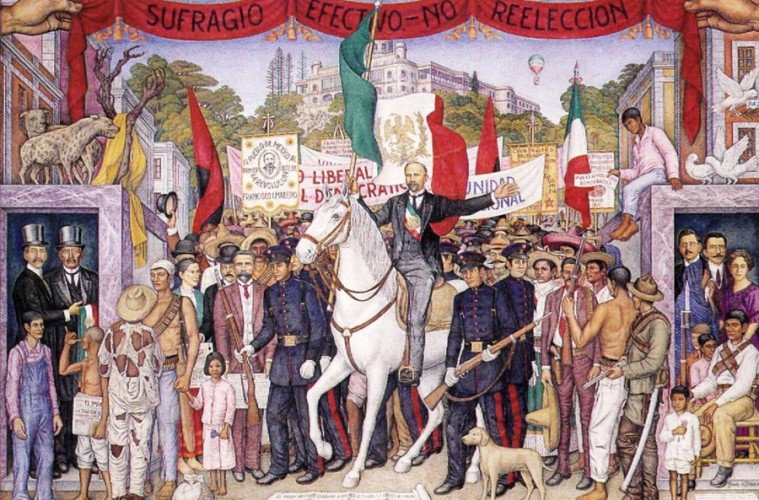
\includegraphics[width=.5\columnwidth]{../../../pics/madero-revo-759x500.jpg} \\
  
  \bigskip

2014: reformers dropped single-term limits for state and federal legislators and municipal governments (effective since 1934)

}
%%%%%%%%%%%%%%%%%%%%%%%%%%%%%%%%%%%%%%%%%%%%%%%%%%%%%%%%%%%%%%%%%%%%%%%%%%%%%%%%%%%%%%%%%%%%%%%%
\frame {                      % SLIDE
\frametitle{The personal vote and familiarity}
Reelection goal $\rightarrow$ credit claiming (Mayhew 1974)

\bigskip

\textbf{But}, with team production of legislation, ascription problems arise

\bigskip \pause

\begin{block}{Cain, Ferejohn, Fiorina (1987)}
  Members prefer particularistic goods (effort/delivery observable)
  \begin{itemize}
  \item constituency service
    \item pork
    \end{itemize}
  %\bigskip %\pause
  $\rightarrow$ cultivate a personal vote and \alert{name familiarity}
  \end{block}

}
%%%%%%%%%%%%%%%%%%%%%%%%%%%%%%%%%%%%%%%%%%%%%%%%%%%%%%%%%%%%%%%%%%%%%%%%%%%%%%%%%%%%%%%%%%%%%%%%
\frame {                      % SLIDE
  \frametitle{Limits of political ambition}
\be
\item Party lock: leaders can veto renomination
\pause
\item Lack of (static) ambition -- cf. Schlesinger
\ee
\bigskip \centering

\begin{tabular}{lcc}
          & & \% returning  \\ \hline
U.S. & {\color{gray}\scriptsize{1990--2010}}      & 86    \\
Chile & {\color{gray}\scriptsize{1993--2000}}     & 59    \\
Brazil & {\color{gray}\scriptsize{1994--2002}}    & 50    \\
Uruguay & {\color{gray}\scriptsize{1985--1999}}   & 34    \\
Colombia & {\color{gray}\scriptsize{1994--2002}}  & 34    \\
\alert<3>{Mexico} & {\color{gray}\scriptsize{2021--2024}}    & \alert<3>{34}    \\
Argentina & {\color{gray}\scriptsize{1983--2001}} & 19    \\ \hline
\end{tabular}

  \bigskip \pause
  
Will removal of single-term limits make any difference?
}
%%%%%%%%%%%%%%%%%%%%%%%%%%%%%%%%%%%%%%%%%%%%%%%%%%%%%%%%%%%%%%%%%%%%%%%%%%%%%%%%%%%%%%%%%%%%%%%%
\frame {                      % SLIDE
  \frametitle{1920s in Mexico}

  Some room for optimism (Godoy 2014)

\bigskip
\centering  
  \begin{tabular}{cr}
            Year &  \% returning \\ \hline
% Const. Congress &          --- \\
            1917 &           18 \\
            1918 &           25 \\
            1920 &           15 \\
            1922 &           26 \\
            1924 &           25 \\
            1926 &           30 \\
            1928 &           40 \\
            1930 &           42 \\
            1932 &           27 \\
            1934 &            0 \\
  \end{tabular}
}
%%%%%%%%%%%%%%%%%%%%%%%%%%%%%%%%%%%%%%%%%%%%%%%%%%%%%%%%%%%%%%%%%%%%%%%%%%%%%%%%%%%%%%%%%%%%%%%%
\frame {                      % SLIDE
\frametitle{The case study}

  \begin{columns}
    \begin{column}{.5\columnwidth}
      Survey evidence of the first election under the new rules: the state assembly of Coahuila in 2017
    \end{column}
  
    \begin{column}{.5\columnwidth}
    \includegraphics[width=\columnwidth]{../../../pics/coa.png} \\
    \end{column}
  \end{columns}

  \bigskip
 Mixed-member system, attention to the 16 SMD races only \\ 3-year terms, 2017 concurrent with gubernatorial election
  
%%   Continuous change in electoral institutions (Molinar 1991)
%%   \begin{description}
%% %  \item Some PR compensation (1964)
%%   \item[1950s] centralization  
%%   \item[1964] compensatory PR
%%   \item[1979] lower entry barriers
%%   \item[1994] PR in Senate
%%   \item[1997] independent Election Board
%%   \item[$\ldots$]
%%   \end{description}
%%   \bigskip
%%   Constant: \alert{single-term limit} across the board since 1934
     }
% %%%%%%%%%%%%%%%%%%%%%%%%%%%%%%%%%%%%%%%%%%%%%%%%%%%%%%%%%%%%%%%%%%%%%%%%%%%%%%%%%%%%%%%%%%%%%%%%
% \frame {                      % SLIDE
%   \frametitle{The 2014 reform}
%   Surprising removal of the consecutive reelection ban
%   \begin{itemize}
%   \item<1> Fed. deputies can reelect up to 4 consecutive three-year terms
%   \item<1> Senators up to 2 consecutive six-year terms
%   \item<1> Incumbent must be re-nominated by same party
%   \item<1> Kick-off: 2021 mid-term
%   \end{itemize}

%   \bigskip \pause
%   Reformers gave states institutional discretion
%   \begin{itemize}
%   \item<2> For state lawmakers: 2-, 3-, or 4-term limits
%   \item<2> For municipal officers: single- or 2-term limits
%   \item<2> Party clause mandatory
%   \item<2> Inapplicable to reformers themselves
%   \end{itemize}
%   \bigskip \pause
%   Variable election calendars $\rightarrow$ incumbents on the ballot \alert{progressively} 
% }
% %%%%%%%%%%%%%%%%%%%%%%%%%%%%%%%%%%%%%%%%%%%%%%%%%%%%%%%%%%%%%%%%%%%%%%%%%%%%%%%%%%%%%%%%%%%%%%%%
% \frame {                      % SLIDE
%   \frametitle{Incumbents on the ballot on July 1st, 2018}

%   \begin{columns}
%   \begin{column}{0.5\textwidth}

%     \begin{block}{State lawmakers only}
%       Aguascalientes,
%       Durango,
%       Hidalgo,
%       Tlaxcala,
%       Veracruz
%     \end{block}

%     \bigskip
%     \begin{block}{Mayors/municipal councils only}
%       Coahuila,
%       Quintana Roo,
%       Tamaulipas
%     \end{block}

%   \end{column}

%       \begin{column}{0.5\textwidth}
%         \begin{block}{Both}
%           Baja California Sur,
%           Campeche,
%           Colima,
%           Chiapas,
%           Chihuahua,
%           Guanajuato,
%           Guerrero,
%           Jalisco,
%           M�xico,
%           Michoac�n,
%           Morelos,
%           Nuevo Le�n,
%           Oaxaca,
%           Quer�taro,
%           San Luis Potos�,
%           Sinaloa,
%           Tabasco,
%           Yucat�n,
%           Zacatecas
%         \end{block}
%       \end{column}
%   \end{columns}
  
%   }
% %%%%%%%%%%%%%%%%%%%%%%%%%%%%%%%%%%%%%%%%%%%%%%%%%%%%%%%%%%%%%%%%%%%%%%%%%%%%%%%%%%%%%%%%%%%%%%%%
% \frame {                      % SLIDE
%   \frametitle{Another obstacle}
%   Pessimists see `party clause' as undermining the electoral connection (Merino et al. 2014)

%   \bigskip \pause
  
%   May be room for maneuver, perhaps a good deal

%   \begin{itemize}
%   \item Two types of candidates: prize fighters and rest (Zaller)
%   \item Party can arrest first type's ambition at its own peril
%   \item Therefore the game is more complex, dual threats
%   \end{itemize}
% }
%%%%%%%%%%%%%%%%%%%%%%%%%%%%%%%%%%%%%%%%%%%%%%%%%%%%%%%%%%%%%%%%%%%%%%%%%%%%%%%%%%%%%%%%%%%%%%%% 
\section{Coahuila 2017}
%%%%%%%%%%%%%%%%%%%%%%%%%%%%%%%%%%%%%%%%%%%%%%%%%%%%%%%%%%%%%%%%%%%%%%%%%%%%%%%%%%%%%%%%%%%%%%%%
\frame {                      % SLIDE
  \frametitle{Coahuila public opinion study}

  Few ambitious members

  \begin{itemize}
  \item 3 deputies re-nominated $\rightarrow$ static ambition
  \item 6 sought municipal presidencies $\rightarrow$ progressive ambition
  \item 16 retired $\rightarrow$ none
  \end{itemize}

  \bigskip

  \begin{columns}
    \begin{column}{.5\columnwidth}
      Moreno: questions on candidate name recognition in May's pre-election survey
    \end{column}
  
    \begin{column}{.5\columnwidth}
    \includegraphics[width=\columnwidth]{../../../pics/portadaFinanciero.png} \\
    \end{column}
  \end{columns}

  
}
%%%%%%%%%%%%%%%%%%%%%%%%%%%%%%%%%%%%%%%%%%%%%%%%%%%%%%%%%%%%%%%%%%%%%%%%%%%%%%%%%%%%%%%%%%%%%%%%
\frame {                      % SLIDE
  \frametitle{Incumbency \emph{v} campaign effects}
  Better name recognition among voters
  \begin{itemize}
  \item Due to incumbent's constituency service and responsiveness?
  \item Or a result of the electoral campaign?
  \end{itemize}
\bigskip \pause
  Three approaches:
  \begin{enumerate}
  \item compare districts with/without incumbent running
  \item compare beginning/end of the campaign
  \item take advantage of \alert<3>{redistricting} to compare voters within constituency
  \end{enumerate}
\bigskip \pause
Geographical groups of voters migrate in/out of districts, candidate name familiarity should vary in predictable ways 
}
% %%%%%%%%%%%%%%%%%%%%%%%%%%%%%%%%%%%%%%%%%%%%%%%%%%%%%%%%%%%%%%%%%%%%%%%%%%%%%%%%%%%%%%%%%%%%%%%%
% \frame {                      % SLIDE
% \frametitle{Inter-election vote swings}
% % $\texttt{Vote swing}_i = f(\texttt{long-term}_i, \texttt{short-term}_i)$
% % \bigskip
% Two effects:
% \begin{itemize}
%   \item incumbency = maintain a pre-existing coalition $\rightarrow$ personal vote (Cain, Ferejohn, Fiorina 1987)  
%   \item campaign = shift existing coalitions (Popkin 1991)  
% \end{itemize}

% \bigskip

% $\rightarrow$ happen simultaneously  

% \bigskip \pause

% Separable with redistricting: geographical groups of voters migrate in/out of districts, candidate name familiarity should vary in predictable ways 
% }
%%%%%%%%%%%%%%%%%%%%%%%%%%%%%%%%%%%%%%%%%%%%%%%%%%%%%%%%%%%%%%%%%%%%%%%%%%%%%%%%%%%%%%%%%%%%%%%% 
\frame {                      % SLIDE
  \frametitle{Using redistricting to separate incumbency effect}
  \centering

\includegraphics[width=.67\columnwidth]{../../../pics/venn-lands.png}

%   \usetikzlibrary{calc}
% \scalebox{.67}{
%     \begin{tikzpicture}
%       \draw (0,0)  ellipse (3 and 2);
%       \node[sloped,above] at ($(0,0)+(90:3 and 2)$) {\emph{dis2014}};
%       \draw (3,0) ellipse (3 and 2);
%       \node[sloped,above] at ($(3,0)+(90:3 and 2)$) {\emph{dis2017}};
%       \draw (-3.5,-3) rectangle (6.5,3);
%       \node [text width=2cm, text centered] at (-1.25,0)   {$l=$ lost}; % p
%       \node [text width=2cm, text centered] at (4.25,0)    {$g=$ gained}; % a
%       \node [text width=2cm, text centered] at (1.5,0)     {$r=$ retained}; % c
%       \node at (1.5,-2.5) {$n=$ no man's land}; % h
%     \end{tikzpicture}
%}

\bigskip \footnotesize{Name recognition expectations}\\
\scalebox{.85}{
\begin{tabular}{ccc}
%    & \mc{2}{c}{Effect} \\ [-.5ex]
    & incumbency & campaign \\ \hline
    1 & \alert<2>{$r>g$}    & \alert<2>{$r=g$}  \\
    2 & $r>l$    & $r>l$  \\
    3 & $r>n$    & $r>n$  \\
    4 & \alert<2>{$l>g$}    & \alert<2>{$l<g$}  \\
    5 & \alert<2>{$l>n$}    & \alert<2>{$l=n$}  \\
    6 & $g>n$    & $g>n$  \\ \hline
\end{tabular} \pause \alert{separation}
}
}
%%%%%%%%%%%%%%%%%%%%%%%%%%%%%%%%%%%%%%%%%%%%%%%%%%%%%%%%%%%%%%%%%%%%%%%%%%%%%%%%%%%%%%%%%%%%%%%% 
\frame {                      % SLIDE
  \frametitle{Few ambitious incumbents}
\resizebox{\linewidth}{!}{
  \begin{tabular}{llcrrrr|rrrr}
                & District/   &                      &  \mc{4}{c}{Secciones}& \mc{4}{c}{Interviewees}  \\ 
    Incumbent    & municipio   & Margin               &  $l$ & $r$ & $g$& $n$  & $l$ & $r$ & $g$ & $n$  \\ \hline
    \hline \\[-1.8ex] 
    \mc{7}{l|}{~~A. \emph{Static ambition (SMD$\rightarrow$SMD)}} \\ \hdashline
  Javier PRI    & Saltillo    &   \color{red}{$-12$} &   14 &  64 & 13 & 1,619 &  14 &  56 &  0  & 938  \\
  Lily PRI      & R. Arispe   & \color{green}{$+14$} &    0 & 117 &  0 & 1,593 &   0 &  56 &  0  & 952  \\
  Gina PRI      & Acu�a       &   \color{red}{$-17$} &    0 &  78 & 21 & 1,611 &   0 &  70 &  0  & 938  \\
  \\[-1.8ex] 
    \mc{7}{l|}{~~B. \emph{Progressive ambition (SMD$\rightarrow$municipio)}} \\ \hdashline
  Lencho PRI    & Frontera    &  \color{green}{$+8$} &   83 &  41 &  0 & 1,586 &  42 &  28 &  0  & 938  \\
  Sonia PRI     & P. Negras   & \color{green}{$+12$} &    0 &  88 &  0 & 1,622 &   0 &  56 &  0  & 952  \\
  AnaIsabel PRI & San Pedro   &  \color{green}{$+3$} &   48 &  75 &  0 & 1,587 &  14 &  42 &  0  & 952  \\ 
  \\[-1.8ex]
  \mc{7}{l|}{~~C. \emph{Progressive ambition (PR$\rightarrow$municipio)}} \\ \hdashline
  Armando PAN   & Frontera    &    \color{red}{$-8$} & 1,635 &  75 &  0 &    0 & 966 &  42 &  0  &   0  \\
  Lariza PAN    & P. Negras   &   \color{red}{$-12$} & 1,635 &  75 &  0 &    0 & 966 &  42 &  0  &   0  \\
  Leonel PPC    & Matamoros   &    \color{red}{$-7$} & 1,648 &  62 &  0 &    0 & 966 &  42 &  0  &   0  \\
  \\[-1.8ex] \hline \hline
  \end{tabular}
}
}
%%%%%%%%%%%%%%%%%%%%%%%%%%%%%%%%%%%%%%%%%%%%%%%%%%%%%%%%%%%%%%%%%%%%%%%%%%%%%%%%%%%%%%%%%%%%%%%%
\frame {                      % SLIDE
  \frametitle{Regression analysis}


  For respondent $i$, we estimate equation
\begin{equation*}
  \begin{split}
\text{logit}(\texttt{recognize}_i) & =    \beta_0
                                       + \beta_1\texttt{retained}_i
                                       + \beta_2\texttt{lost}_i \\
                                       + \beta_3\texttt{delivered}_i 
                                     & + \beta_4\texttt{interested}_i
                                       + \beta_5\texttt{smartphone}_i \\ 
                                       + \beta_6\texttt{panista}_i 
                                     & + \beta_7\texttt{priista}_i
                                       + \beta_8\texttt{morenista}_i
                                       + \text{error}_i.
  \end{split}
\end{equation*}
}
%%%%%%%%%%%%%%%%%%%%%%%%%%%%%%%%%%%%%%%%%%%%%%%%%%%%%%%%%%%%%%%%%%%%%%%%%%%%%%%%%%%%%%%%%%%%%%%%
\frame {                      % SLIDE
  \frametitle{Results}
  \scalebox{.5}{
\begin{tabular}{l|rrr|rrr|rrr} 
\\[-1.8ex] & \multicolumn{1}{c}{(1)} & \multicolumn{1}{c}{(2)} & \multicolumn{1}{c}{(3)} & \multicolumn{1}{c}{(4)} & \multicolumn{1}{c}{(5)} & \multicolumn{1}{c}{(6)} & \multicolumn{1}{c}{(7)} & \multicolumn{1}{c}{(8)} & \multicolumn{1}{c}{(9)}\\ 
  & \multicolumn{1}{c}{Javier} & \multicolumn{1}{c}{Lily} & \multicolumn{1}{c}{Gina} & \multicolumn{1}{c}{Lencho} & \multicolumn{1}{c}{Sonia} & \multicolumn{1}{c}{A.Isabel} & \multicolumn{1}{c}{Armando} & \multicolumn{1}{c}{Lariza} & \multicolumn{1}{c}{Leonel}\\ 
\hline \\[-1.8ex] 
 $\texttt{retained}$   & 1.85^{***} & 2.37^{***} & 4.91^{***} & 3.10^{***} & 3.02^{***} & 4.59^{***} & 1.10^{*} & -.22 & 2.93^{***} \\ 
  & (.33) & (.33) & (.41) & (.43) & (.32) & (.44) & (.58) & (.75) & (.38) \\ 
  & & & & & & & & & \\ 
 $\texttt{lost}$       & 1.29^{*} &  &  & 1.27^{***} &  & 1.46^{*} &  &  &  \\ 
  & (.68) &  &  & (.47) &  & (.81) &  &  &  \\ 
  & & & & & & & & & \\ 
 $\texttt{delivered}$  & .86^{***} & .76^{***} & 1.46^{***} & .51^{*} & .93^{***} & .26 & .51 & .85^{***} & .26 \\ 
  & (.25) & (.27) & (.34) & (.30) & (.27) & (.34) & (.37) & (.27) & (.33) \\ 
  & & & & & & & & & \\ 
 $\texttt{interested}$ & .35 & 1.03^{***} & 1.34^{***} & .82^{***} & .52^{**} & .74^{**} & .71^{**} & .28 & .57^{*} \\ 
  & (.24) & (.27) & (.34) & (.28) & (.26) & (.33) & (.36) & (.27) & (.31) \\ 
  & & & & & & & & & \\ 
 $\texttt{smartphone}$ & -.27 & .37 & -.18 & -.47^{*} & .21 & -.05 & -.43 & .26 & -.42 \\ 
  & (.24) & (.27) & (.31) & (.28) & (.26) & (.31) & (.35) & (.27) & (.30) \\ 
  & & & & & & & & & \\ 
 $\texttt{panista}$    & .15 & -.11 & -.03 & 1.18^{***} & .02 & .80^{*} & .78^{*} & .34 & 1.15^{***} \\ 
  & (.39) & (.41) & (.52) & (.35) & (.41) & (.44) & (.47) & (.39) & (.41) \\ 
  & & & & & & & & & \\ 
 $\texttt{priista}$    & .37 & .15 & -.01 & -.21 & .17 & .74^{**} & .43 & .19 & .16 \\ 
  & (.28) & (.30) & (.38) & (.37) & (.29) & (.35) & (.41) & (.31) & (.39) \\ 
  & & & & & & & & & \\ 
 $\texttt{morenista}$  & -.07 & .59 & .26 & .76 & -1.17 &  & -.26 & -1.01 & .88 \\ 
  & (.63) & (.51) & (.74) & (.55) & (1.04) &  & (1.05) & (1.03) & (.56) \\ 
  & & & & & & & & & \\ 
 Intercept             & -3.03^{***} & -3.82^{***} & -4.45^{***} & -3.48^{***} & -3.49^{***} & -3.99^{***} & -3.87^{***} & -3.29^{***} & -3.58^{***} \\ 
  & (.25) & (.30) & (.39) & (.30) & (.28) & (.35) & (.37) & (.28) & (.30) \\ 
  & & & & & & & & & \\ 
\hline \\[-1.8ex] 
Observations & \multicolumn{1}{c}{1,008} & \multicolumn{1}{c}{1,008} & \multicolumn{1}{c}{1,008} & \multicolumn{1}{c}{1,008} & \multicolumn{1}{c}{1,008} & \multicolumn{1}{c}{1,008} & \multicolumn{1}{c}{1,008} & \multicolumn{1}{c}{1,008} & \multicolumn{1}{c}{1,008} \\ 
Log Likelihood & \multicolumn{1}{c}{-262.32} & \multicolumn{1}{c}{-231.34} & \multicolumn{1}{c}{-169.84} & \multicolumn{1}{c}{-205.60} & \multicolumn{1}{c}{-235.20} & \multicolumn{1}{c}{-175.64} & \multicolumn{1}{c}{-147.10} & \multicolumn{1}{c}{-229.85} & \multicolumn{1}{c}{-182.89} \\ 
\hline 
\hline \\[-1.8ex] 
    \multicolumn{10}{r}{\footnotesize{$^{*}$p$<$.1; $^{**}$p$<$.05; $^{***}$p$<$.01}} \\ %[-1.8ex]
\end{tabular} 
    }
}
%%%%%%%%%%%%%%%%%%%%%%%%%%%%%%%%%%%%%%%%%%%%%%%%%%%%%%%%%%%%%%%%%%%%%%%%%%%%%%%%%%%%%%%%%%%%%%%%
\frame {                      % SLIDE
  \frametitle{Results (name recognition in x-axis)}
\centering
  \resizebox{\linewidth}{!}{
  \begin{tabular}{ccc}
    Static ambition & Progressive ambition SMD & Progressive ambition PR \\ \hline
    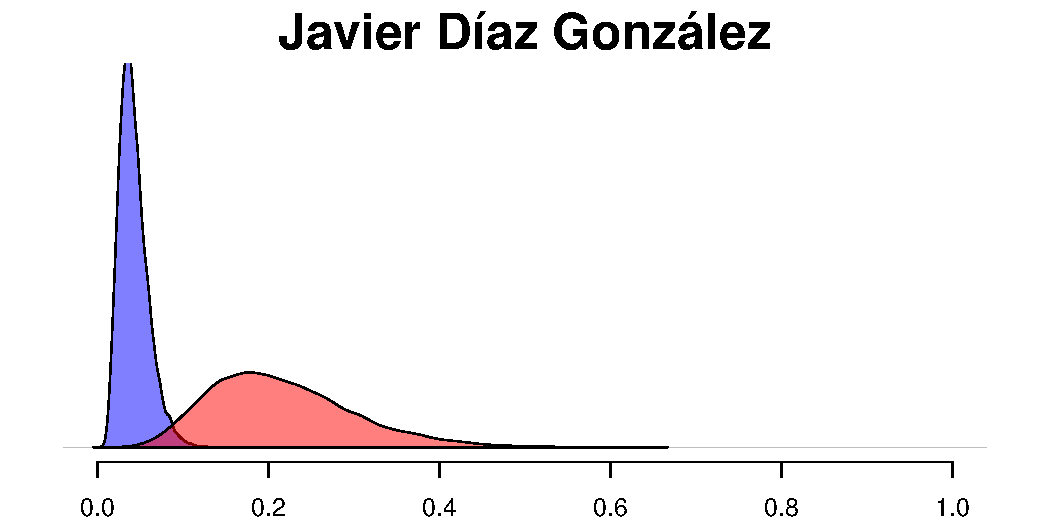
\includegraphics[width=.3\columnwidth]{../../graphs/prReconoce1.pdf} &
    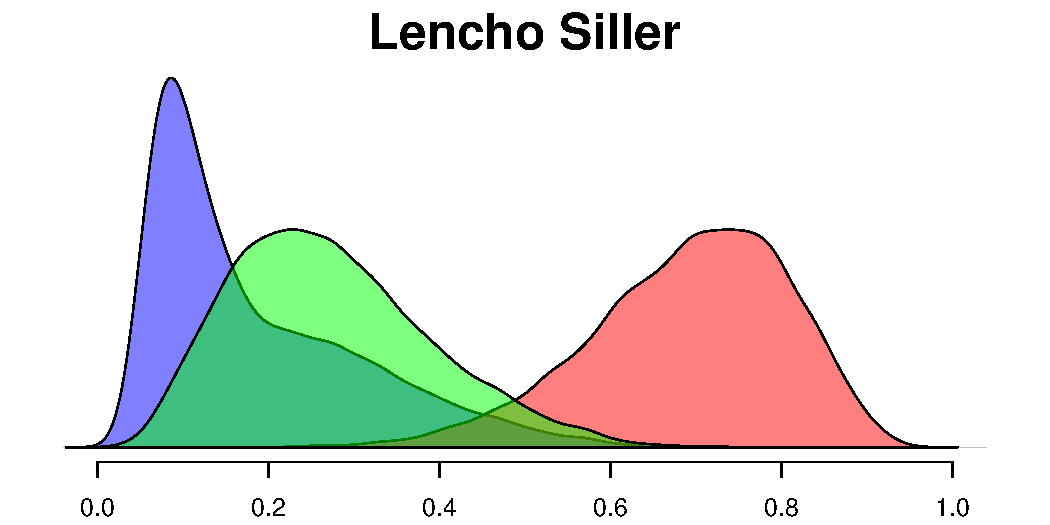
\includegraphics[width=.3\columnwidth]{../../graphs/prReconoce6.pdf} &
    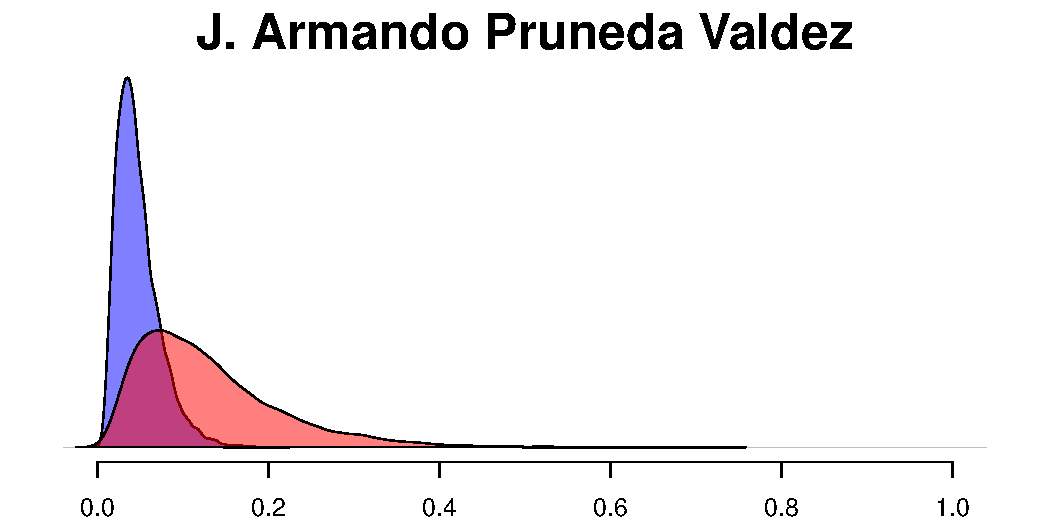
\includegraphics[width=.3\columnwidth]{../../graphs/prReconoce8.pdf} \\
    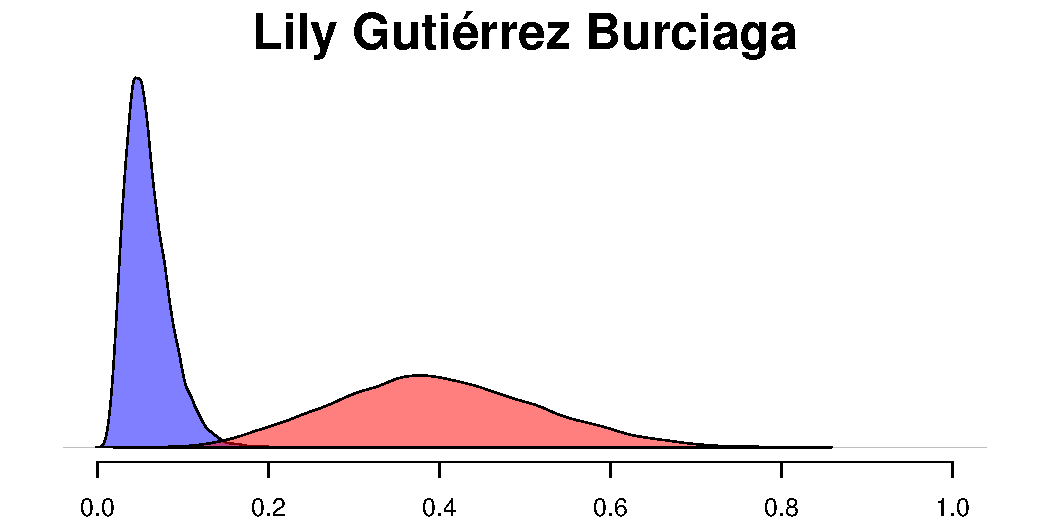
\includegraphics[width=.3\columnwidth]{../../graphs/prReconoce2.pdf} &
    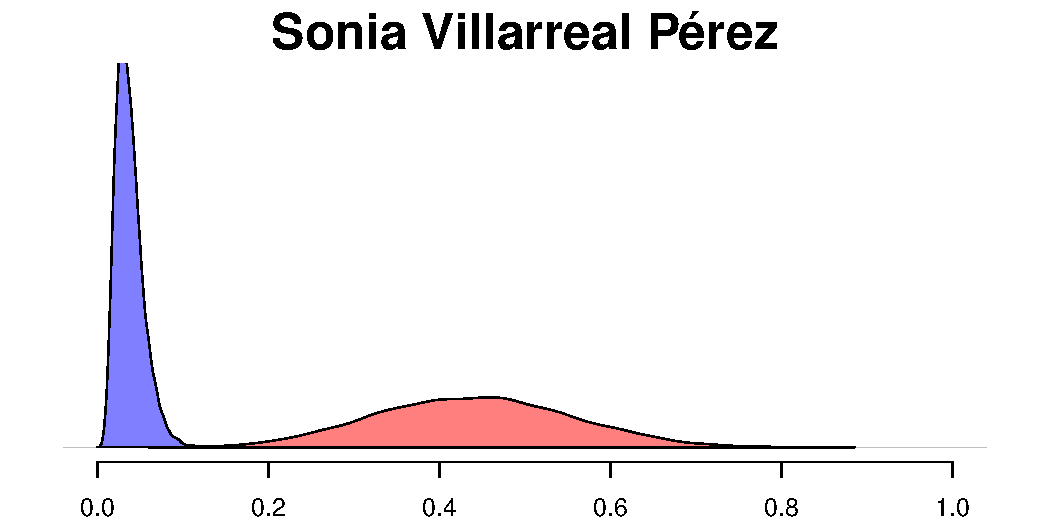
\includegraphics[width=.3\columnwidth]{../../graphs/prReconoce5.pdf} &
    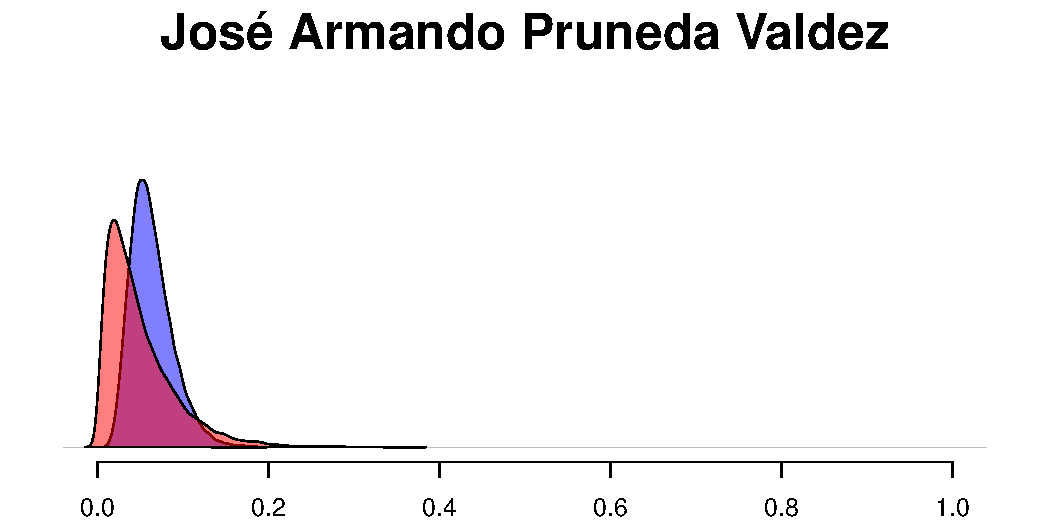
\includegraphics[width=.3\columnwidth]{../../graphs/prReconoce7.pdf} \\
    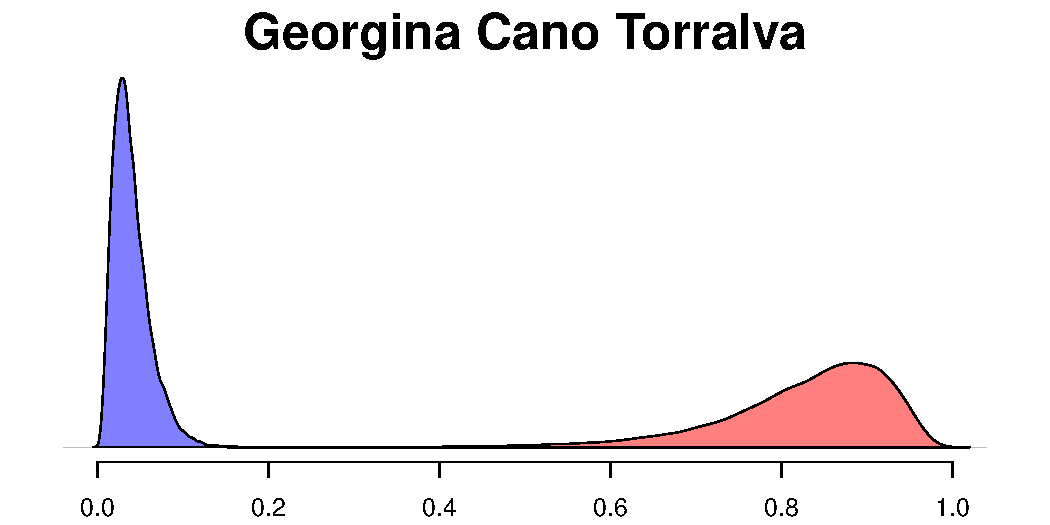
\includegraphics[width=.3\columnwidth]{../../graphs/prReconoce3.pdf} &
    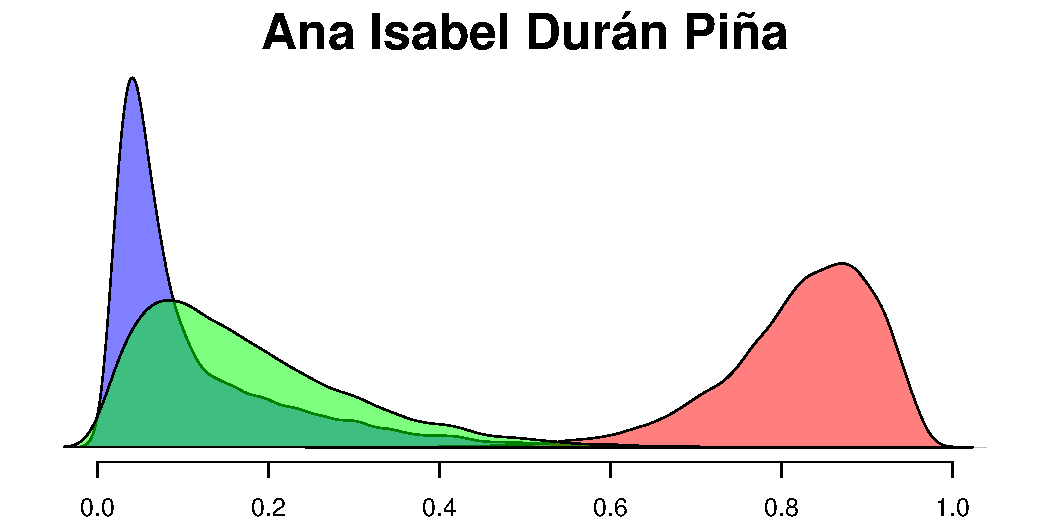
\includegraphics[width=.3\columnwidth]{../../graphs/prReconoce4.pdf} &
    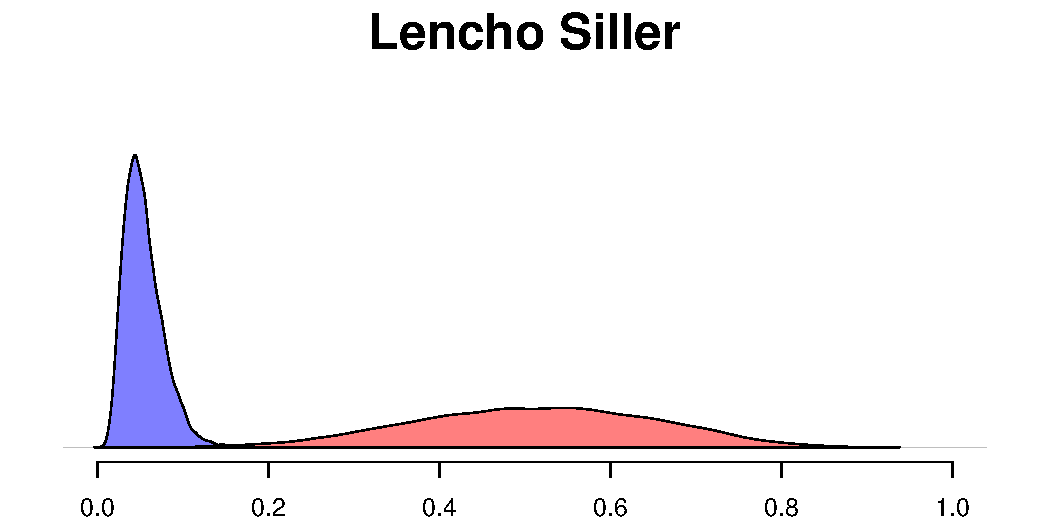
\includegraphics[width=.3\columnwidth]{../../graphs/prReconoce9.pdf} \\
  \end{tabular}
}

\bigskip

Hypotheses:
\begin{tabular}{rc}
  incumbency & \textcolor{MidnightBlue}{$n$} $<$ \textcolor{LimeGreen}{$l$} $<$ \textcolor{Salmon}{$r$} \\
  campaign   & \textcolor{MidnightBlue}{$n$} $=$ \textcolor{LimeGreen}{$l$} $<$ \textcolor{Salmon}{$r$} \\
\end{tabular}
}
%%%%%%%%%%%%%%%%%%%%%%%%%%%%%%%%%%%%%%%%%%%%%%%%%%%%%%%%%%%%%%%%%%%%%%%%%%%%%%%%%%%%%%%%%%%%%%%%
\frame {                      % SLIDE
  \frametitle{Hypothesis tests}
\centering
  \begin{tabular}{lrrr}
                          & \multicolumn{3}{c}{Hypothesis} \\
  Model and incumbent     & $r>n$ & $l>n$ & $r>l$ \\ \hline
  \multicolumn{4}{l}{\textbf{~~~SMD, static ambition}} \\
1 Javier D�az Gonz�lez    & \color{green}{$<.001$} & \color{green}{$.029$} & \color{red}{$.221$} \\
2 Lily Guti�rrez Burciaga & \color{green}{$<.001$} & ---    & --- \\
3 Gina Cano Torralva      & \color{green}{$<.001$} & ---    & --- \\ \hline
\end{tabular}
}
%%%%%%%%%%%%%%%%%%%%%%%%%%%%%%%%%%%%%%%%%%%%%%%%%%%%%%%%%%%%%%%%%%%%%%%%%%%%%%%%%%%%%%%%%%%%%%%%
\frame {                      % SLIDE
  \frametitle{Hypothesis tests}
\centering
  \begin{tabular}{lrrr}
                          & \multicolumn{3}{c}{Hypothesis} \\
  Model and incumbent     & $r>n$ & $l>n$ & $r>l$ \\ \hline
  \multicolumn{4}{l}{\textbf{~~~SMD, progressive ambition}} \\
4 Lencho Siller           & \color{green}{$<.001$} & \color{green}{$.003$} & \color{green}{$.001$} \\
5 Sonia Villarreal P�rez  & \color{green}{$<.001$} & ---    & --- \\
6 Ana Isabel Dur�n Pi�a   & \color{green}{$<.001$} & \color{green}{$.036$} & \color{green}{$<.001$} \\
  \multicolumn{4}{l}{\textbf{~~~PR, progressive ambition}} \\
7 Armando Pruneda Valdez  & \color{green}{$.030$}  & ---    & --- \\
8 Lariza Montiel Luis     & \color{red}{$.385$}    & ---    & --- \\
9 Leonel Contreras P�manes& \color{green}{$<.001$} & ---    & --- \\ \hline
\end{tabular}
}
%%%%%%%%%%%%%%%%%%%%%%%%%%%%%%%%%%%%%%%%%%%%%%%%%%%%%%%%%%%%%%%%%%%%%%%%%%%%%%%%%%%%%%%%%%%%%%%%
\section{Conclusion}
%%%%%%%%%%%%%%%%%%%%%%%%%%%%%%%%%%%%%%%%%%%%%%%%%%%%%%%%%%%%%%%%%%%%%%%%%%%%%%%%%%%%%%%%%%%%%%%%
\frame {                      % SLIDE
  \frametitle{Wrap-up}
  \begin{itemize}
  \item Survey evidence consistent with incumbency effect, \\ but can't fully rule out campaign
  \item Separation needs more incumbents on the ballot
  \item Next step: municipal elections in 2022, two surveys
  \item Whether or not the reelection potential fulfilled = promising research area in Mexican politics
  \end{itemize}
  \pause \bigskip \centering 
  \textbf{Thank you!}
}

\end{document}
